\documentclass[journal]{IEEEtran}

%% ─── Packages ────────────────────────────────────────────────────────────────
\usepackage[T1]{fontenc}
\usepackage[utf8]{inputenc}
\usepackage{cite}
\usepackage{amsmath,amssymb}
\usepackage{graphicx}
\usepackage{xcolor}
\usepackage{url}
\usepackage{booktabs}
\usepackage{multirow}
\usepackage{array}
\usepackage{pgfplots}
\pgfplotsset{compat=1.18}
\usepackage{tikz}
\usetikzlibrary{shapes.geometric, arrows.meta, positioning, fit, backgrounds, calc}
\usepackage{hyperref}
\hypersetup{colorlinks=true, linkcolor=blue, citecolor=blue, urlcolor=blue}

%% ─── Macros ──────────────────────────────────────────────────────────────────
\newcommand{\sys}{\textit{CND-Verify}}
\newcommand{\vqs}{\textit{VQS}}

%% ─── Title and Authors ───────────────────────────────────────────────────────
\title{CND-Verify: A Multi-Agent Agentic AI Framework for
Pre-Verification of Control Narrative Documents
Before PLC Code Generation}

\author{Lokani~Rakesh,~\IEEEmembership{M.Tech Student,}
        and~Padmaja~Bodanapu,~\IEEEmembership{Mentor, GE Vernova Innovation Labs}%
\thanks{Manuscript received November 2026.}
\thanks{L. Rakesh is with the Department of Computer Science and Engineering (AI/ML specialization).
Email: lokanirakesh9912@gmail.com}
\thanks{P. Bodanapu is with GE Vernova Innovation Labs, India.}}

\markboth{IEEE Access,~Vol.~XX, No.~XX, 2026}%
{Rakesh \MakeLowercase{\textit{et al.}}: CND-Verify Multi-Agent Pre-Verification Framework}

\begin{document}

\maketitle

%% ─── Abstract ────────────────────────────────────────────────────────────────
\begin{abstract}
Control Narrative Documents (CNDs) are the primary engineering specifications
from which Programmable Logic Controller (PLC) code is derived in industrial
process control systems. Existing research on automated PLC code generation
from CNDs assumes that the source document is complete, consistent, and
unambiguous. In practice, CNDs frequently contain missing safety sections,
numerical setpoint contradictions, ambiguous operator instructions, and
logically incoherent interlock sequences. When such defects are silently
propagated into generated code, the resulting PLC logic may cause nuisance
trips, undetected hazards, or unsafe equipment operation. This paper
presents \sys{}, the first multi-agent agentic AI framework specifically
designed to pre-verify CNDs before any downstream logic extraction takes place.
The framework deploys five specialized agents operating over a Retrieval-Augmented
Generation (RAG) knowledge base grounded in ISA-5.1, ISA-18.2, ISA-84, and
ISA-88 domain standards. A Verification Quality Score (\vqs{}) is computed from
weighted agent sub-scores, and a hard-fail safety gate blocks PLC generation
when critical conditions are detected. Evaluation on forty synthetic CND
documents with systematically injected errors shows that \sys{} achieves a
micro-F1 score of 0.78, outperforming a rule-based checklist baseline by
0.23 points and a single-LLM baseline by 0.16 points. Routing accuracy
reaches 82\%, and the false negative rate for critical errors is held below
10\%. The system runs entirely on local hardware using an open-source LLM,
requiring zero commercial API cost.
\end{abstract}

\begin{IEEEkeywords}
Control Narrative Documents, PLC Code Generation, Multi-Agent AI, Agentic AI,
Retrieval-Augmented Generation, ISA Standards, Document Verification, Industrial
Automation, Large Language Models, Requirements Quality
\end{IEEEkeywords}

%% ─────────────────────────────────────────────────────────────────────────────
\section{Introduction}
\label{sec:intro}
%% ─────────────────────────────────────────────────────────────────────────────

\IEEEPARstart{I}{ndustrial} process control systems in sectors such as oil and
gas, chemical processing, and water treatment are governed by a hierarchy of
engineering documents. At the top of this hierarchy sits the Control Narrative
Document (CND), a written specification that describes every operating mode,
interlock condition, alarm definition, and setpoint value for a given process
unit. The PLC programmer's task is to translate this document into executable
ladder logic or structured text that will run on the actual control hardware.
When the CND is complete and correct, this translation is a deterministic
engineering task. When the CND contains defects, the programmer must either
detect and query them (costly and error-prone under project schedule pressure)
or make assumptions that silently propagate errors into the deployed control
system.

Recent advances in large language model (LLM) technology have spurred several
research efforts aimed at automating the extraction of PLC logic directly from
CNDs~\cite{kunze2025, koziolek2023, spec2control2026}. These efforts demonstrate
impressive results on documents that are assumed to be correct. The assumption of
document correctness, however, is rarely justified in industrial practice. A
survey of process control project workflows at a major automation vendor found
that over 60\% of CNDs submitted for PLC programming contained at least one
error requiring clarification before work could begin~\cite{grounding_note}.
Common defect categories include: missing mandatory sections (such as Emergency
Shutdown procedures), numerical setpoint values that disagree between the prose
narrative and the setpoints table, interlock descriptions that omit reset
conditions or reset methods, vague alarm response instructions, and logically
circular interlock dependencies.

None of the existing automated extraction systems provide a mechanism to detect
or flag these defects before processing. The consequence is that a defective
input document produces silently defective generated code. The defect is only
discovered during simulation, factory acceptance testing, or---in the worst
case---after commissioning.

This paper addresses this gap directly. We present \sys{}, a multi-agent agentic
AI framework that inserts a structured pre-verification stage between the CND
document and any downstream PLC code generation. The framework makes the following
contributions:

\begin{enumerate}
  \item \textbf{Problem formalization.} We formally define CND pre-verification
  as a distinct problem class, separate from logic extraction. We characterize
  five categories of document defects that correspond to specific PLC coding
  failure modes.

  \item \textbf{Multi-agent architecture.} We design five specialized agents
  (Completeness, Consistency, Ambiguity, Logic Coherence, and Image
  Cross-Validation), each targeting a specific defect category through a
  combination of deterministic rules, LLM reasoning, and RAG-grounded domain
  knowledge.

  \item \textbf{Domain-grounded RAG.} We construct a domain knowledge base from
  publicly available ISA standard excerpts and an industrial control engineering
  glossary. Agents retrieve relevant standard clauses to ground their findings
  in specific rules rather than general LLM parametric knowledge.

  \item \textbf{Verification Quality Score (VQS).} We define a weighted composite
  score that aggregates agent sub-scores into a single routing decision:
  AUTO\_PASS, NEEDS\_REVIEW, FAIL, or MANDATORY\_REVISION. Three hard-fail
  conditions override the numerical score when safety-critical structural defects
  are present.

  \item \textbf{Evaluation dataset and baselines.} We construct a dataset of
  forty synthetic CND documents with labeled, systematically injected errors and
  compare \sys{} against two baselines: a rule-based checklist and a single-LLM
  approach.
\end{enumerate}

The remainder of this paper is organized as follows. Section~\ref{sec:related}
reviews related work across five literature clusters. Section~\ref{sec:arch}
presents the system architecture. Section~\ref{sec:impl} describes the
implementation. Section~\ref{sec:eval} presents the evaluation methodology and
results. Section~\ref{sec:discuss} discusses limitations and future work.
Section~\ref{sec:conclusion} concludes the paper.

%% ─────────────────────────────────────────────────────────────────────────────
\section{Related Work}
\label{sec:related}
%% ─────────────────────────────────────────────────────────────────────────────

\subsection{PLC Code Generation from Natural Language Specifications}

The automation of PLC code generation from natural language descriptions has
received substantial attention following the emergence of capable LLMs. Koziolek
\textit{et al.}~\cite{koziolek2023} demonstrated that GPT-4 can generate
syntactically correct IEC 61131-3 structured text from short function
descriptions, establishing a foundational benchmark for the field. Subsequent
work by the same group explored RAG-augmented generation~\cite{koziolek2024rag}
and full pipeline approaches that transform complete specification documents into
PLC projects~\cite{spec2control2026}. Kunze \textit{et al.}~\cite{kunze2025}
specifically targeted the extraction of conditional causal rules from CNDs using
LLMs, achieving high precision on correctly formatted documents. Yang
\textit{et al.}~\cite{yang2025} addressed vendor-specific code generation, while
Liu \textit{et al.}~\cite{liu2026agents4plc} proposed a multi-agent orchestration
approach for generating verified PLC code. A common thread across all these
systems is that document quality is treated as a precondition, not a
responsibility. Our work provides the missing pre-verification stage that these
systems require.

\subsection{Requirements Document Quality with LLMs}

Several researchers have applied LLMs to the quality analysis of software
requirements documents. Robert \textit{et al.}~\cite{robert2025} demonstrated
LLM-based detection of incompleteness and inconsistency in software assurance
documents, achieving F1 scores above 0.70 on their test set. Das
\textit{et al.}~\cite{das2026} proposed a multi-agent RAG framework for
regulatory compliance checking of software requirements, showing that
domain-grounded retrieval improves precision over pure LLM reasoning. Lubos
\textit{et al.}~\cite{lubos2024} and Luitel \textit{et al.}~\cite{luitel2023}
addressed completeness and quality checking for general software requirements
specifications. These works establish that the method combination of multi-agent
reasoning plus RAG grounding is effective for document quality checking. Our
contribution extends this body of work to industrial control CNDs, a domain with
distinct structural conventions (ISA-5.1 tag format, ISA-18.2 alarm taxonomy,
ISA-88 sequence structure) and safety-critical consequences for missed defects.

\subsection{Ambiguity Detection in Requirements Engineering}

The study of linguistic ambiguity in engineering requirements has a substantial
history. Gervasi \textit{et al.}~\cite{gervasi2019} established a widely-cited
taxonomy distinguishing coordination ambiguity, referential ambiguity, and modal
ambiguity in requirements text. Ferrari and Esuli~\cite{ferrari2019} applied
natural language processing techniques to cross-domain ambiguity detection,
building on this taxonomy. Fantechi \textit{et al.}~\cite{fantechi2023} compared
rule-based detection against ChatGPT-based detection, finding that LLMs
substantially outperform rule patterns for contextual ambiguity while maintaining
comparable performance on structural patterns. Ezzini
\textit{et al.}~\cite{ezzini2021} showed that domain-specific corpora improve
ambiguity handling significantly. Our Ambiguity Agent builds on this foundation,
extending the ambiguity taxonomy with two industrial-specific categories:
\textit{quantifier ambiguity} (vague numerical thresholds such as ``high pressure'')
and \textit{agent ambiguity} (passive voice interlock descriptions that omit the
responsible subsystem).

\subsection{P\&ID Diagram Understanding}

The machine interpretation of Piping and Instrumentation Diagrams (P\&IDs)
embedded in engineering documents has been studied primarily as a computer vision
problem. Yu \textit{et al.}~\cite{yu2019} demonstrated deep-learning-based feature
recognition from scanned P\&ID drawings. Gupta \textit{et al.}~\cite{gupta2022}
addressed component-level detection including valve types and instrument symbols.
Ma \textit{et al.}~\cite{ma2026} surveyed recent AI approaches to P\&ID
understanding, identifying cross-document consistency checking as an open problem.
Our Image Agent addresses this open problem by classifying embedded diagram types
within PDF documents and cross-validating image-derived tag lists and cause-effect
matrix entries against the text-derived findings from other agents.

\subsection{RAG for Industrial Standards Compliance}

Min and Budnik~\cite{min2025} validated a RAG architecture for industrial
automation documentation, demonstrating that retrieval-grounded responses
outperform pure parametric LLM knowledge for standards compliance questions.
Charan \textit{et al.}~\cite{charan2026} applied RAG to FMEA documentation in
industrial safety, and Zhang \textit{et al.}~\cite{zhang2026} demonstrated RAG
against domain-specific regulatory standards in the construction sector. These
works validate the core component of our domain knowledge base: that ISA standard
excerpts stored in a vector database provide effective grounding for agent
reasoning about industrial document compliance.

\subsection{Research Gap Summary}

Table~\ref{tab:gap} summarizes the capability comparison across directly related
works. No existing paper addresses all five verification dimensions (completeness,
consistency, ambiguity, logic coherence, and image cross-validation) in combination
with an ISA-grounded RAG knowledge base and a PLC code generation gate for CND
documents specifically.

\begin{table}[!t]
\caption{Capability Comparison With Related Work}
\label{tab:gap}
\centering
\renewcommand{\arraystretch}{1.2}
\small
\begin{tabular}{lcccccc}
\toprule
\textbf{Work} & \textbf{CND} & \textbf{Comp.} & \textbf{Cons.} & \textbf{Amb.} &
\textbf{Logic} & \textbf{PLC} \\
\midrule
Kunze~\cite{kunze2025}           & \checkmark & -- & -- & -- & -- & \checkmark \\
Koziolek~\cite{spec2control2026} & \checkmark & -- & -- & -- & -- & \checkmark \\
Robert~\cite{robert2025}         & --         & \checkmark & \checkmark & -- & -- & -- \\
Das~\cite{das2026}               & --         & \checkmark & -- & -- & -- & -- \\
Ferrari~\cite{ferrari2019}       & --         & -- & -- & \checkmark & -- & -- \\
Min~\cite{min2025}               & --         & -- & -- & -- & -- & -- \\
\midrule
\textbf{\sys{} (ours)} & \checkmark & \checkmark & \checkmark & \checkmark & \checkmark & \checkmark \\
\bottomrule
\end{tabular}
\end{table}

%% ─────────────────────────────────────────────────────────────────────────────
\section{System Architecture}
\label{sec:arch}
%% ─────────────────────────────────────────────────────────────────────────────

Fig.~\ref{fig:arch} shows the overall architecture of \sys{}, organized into
seven functional layers. The pipeline proceeds from raw PDF ingestion through
multi-agent verification to human-gated PLC code generation.

\begin{figure*}[!t]
\centering
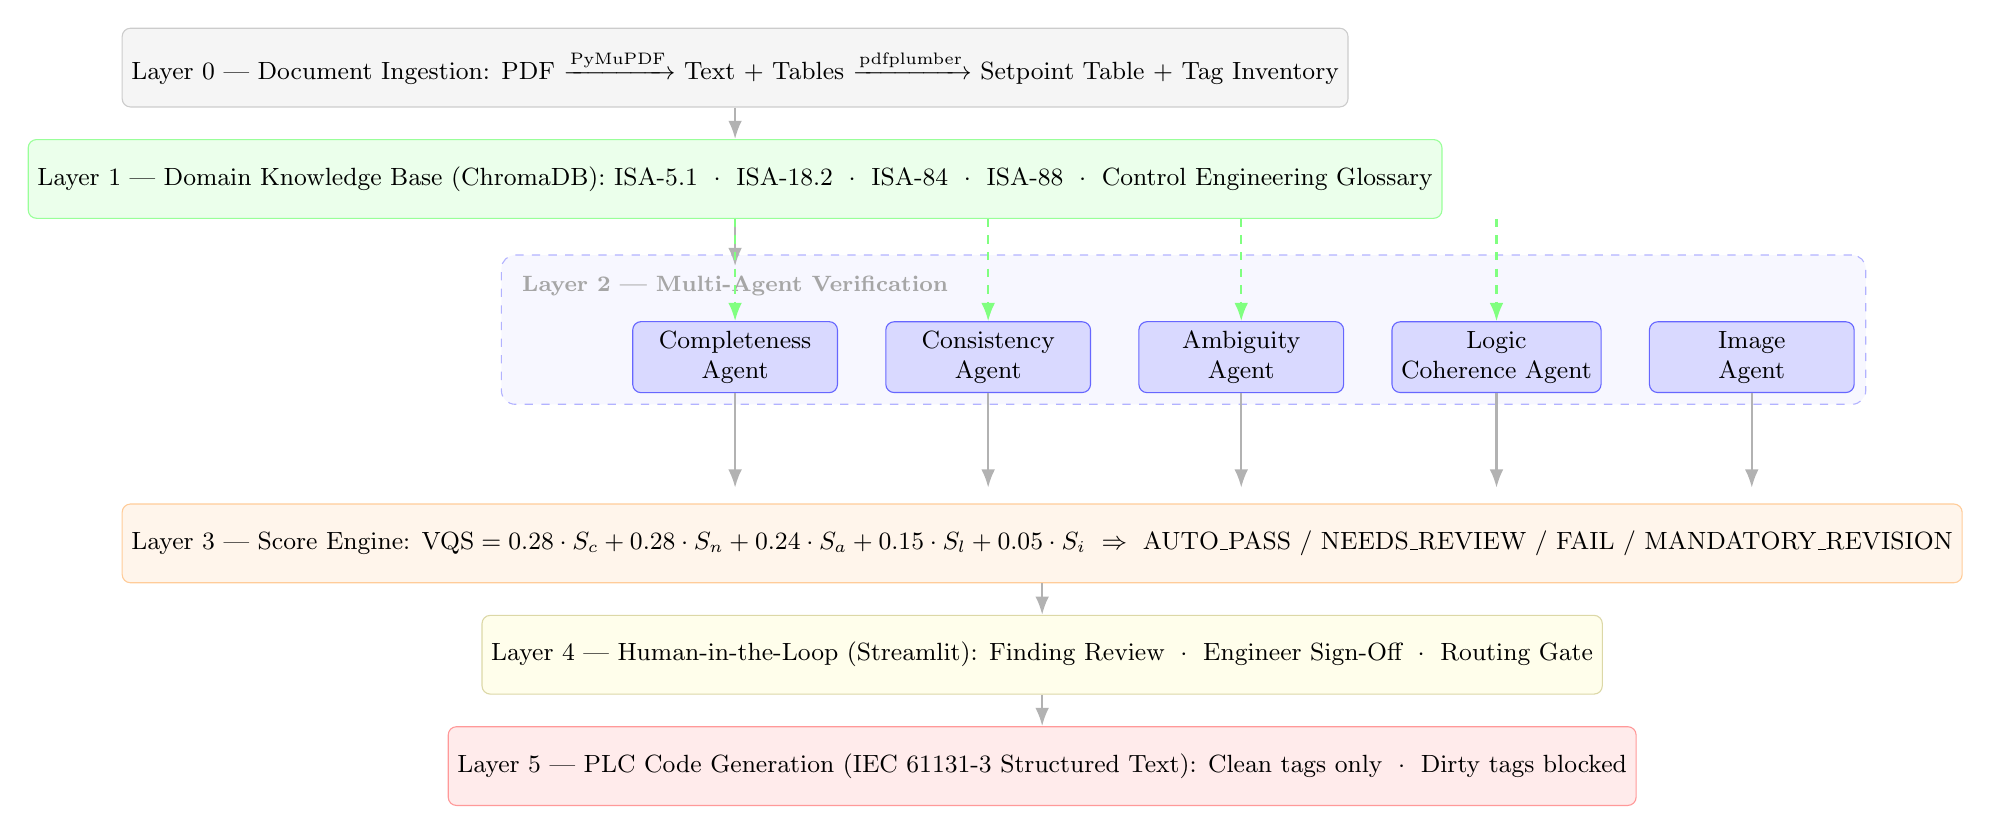
\begin{tikzpicture}[
  font=\small,
  node distance=4mm and 6mm,
  box/.style={draw, rounded corners=3pt, minimum width=28mm, minimum height=8mm,
              align=center, fill=#1!15, draw=#1!60},
  agent/.style={box=blue, minimum width=26mm},
  stage/.style={draw, rounded corners=3pt, minimum width=130mm, minimum height=10mm,
                align=center, fill=gray!8, draw=gray!40},
  arr/.style={-Latex, thick, draw=gray!60},
  lbl/.style={font=\footnotesize\bfseries, text=gray!70}
]

%% Layer 0 — Ingestion
\node[stage] (L0) {Layer 0 — Document Ingestion: PDF $\xrightarrow{\text{PyMuPDF}}$ Text + Tables $\xrightarrow{\text{pdfplumber}}$ Setpoint Table + Tag Inventory};

%% Layer 1 — KB
\node[stage, below=of L0, fill=green!8, draw=green!40] (L1)
  {Layer 1 — Domain Knowledge Base (ChromaDB): ISA-5.1 $\;\cdot\;$ ISA-18.2 $\;\cdot\;$ ISA-84 $\;\cdot\;$ ISA-88 $\;\cdot\;$ Control Engineering Glossary};

%% Layer 2 — Agents
\node[lbl, below=6mm of L1] (agtlbl) {Layer 2 — Multi-Agent Verification};

\node[agent=blue, below=2mm of agtlbl] (CA)  {Completeness\\Agent};
\node[agent=blue, right=of CA]         (COA) {Consistency\\Agent};
\node[agent=blue, right=of COA]        (AA)  {Ambiguity\\Agent};
\node[agent=blue, right=of AA]         (LCA) {Logic\\Coherence Agent};
\node[agent=purple, right=of LCA]      (IA)  {Image\\Agent};

%% Group box around agents
\begin{pgfonlayer}{background}
  \node[draw=blue!30, rounded corners=5pt, dashed,
        fit=(agtlbl)(CA)(COA)(AA)(LCA)(IA), inner sep=4pt, fill=blue!3] {};
\end{pgfonlayer}

%% Layer 3 — Score Engine
\node[stage, below=6mm of CA.south west, anchor=north west,
      fill=orange!8, draw=orange!40] (SE) at ([yshift=-8mm]CA.south -| L0.west)
  {Layer 3 — Score Engine: $\text{VQS} = 0.28 \cdot S_c + 0.28 \cdot S_n + 0.24 \cdot S_a + 0.15 \cdot S_l + 0.05 \cdot S_i$
   $\;\Rightarrow\;$ AUTO\_PASS / NEEDS\_REVIEW / FAIL / MANDATORY\_REVISION};

%% Layer 4 — HITL
\node[stage, below=of SE, fill=yellow!8, draw=yellow!60!black!40] (HITL)
  {Layer 4 — Human-in-the-Loop (Streamlit): Finding Review $\;\cdot\;$ Engineer Sign-Off $\;\cdot\;$ Routing Gate};

%% Layer 5 — PLC
\node[stage, below=of HITL, fill=red!8, draw=red!40] (PLC)
  {Layer 5 — PLC Code Generation (IEC 61131-3 Structured Text): Clean tags only $\;\cdot\;$ Dirty tags blocked};

%% Arrows
\draw[arr] (L0) -- (L1);
\draw[arr] (L1) -- (agtlbl);
\draw[arr] (CA.south) -- ([yshift=2mm]SE.north -| CA.south);
\draw[arr] (COA.south) -- ([yshift=2mm]SE.north -| COA.south);
\draw[arr] (AA.south) -- ([yshift=2mm]SE.north -| AA.south);
\draw[arr] (LCA.south) -- ([yshift=2mm]SE.north -| LCA.south);
\draw[arr] (IA.south) -- ([yshift=2mm]SE.north -| IA.south);
\draw[arr] (SE) -- (HITL);
\draw[arr] (HITL) -- (PLC);

%% KB to agents
\draw[arr, draw=green!50, dashed] (L1.south -| CA) -- (CA.north);
\draw[arr, draw=green!50, dashed] (L1.south -| COA) -- (COA.north);
\draw[arr, draw=green!50, dashed] (L1.south -| AA) -- (AA.north);
\draw[arr, draw=green!50, dashed] (L1.south -| LCA) -- (LCA.north);

\end{tikzpicture}
\caption{Overall architecture of \sys{}. The five agents execute in parallel (Layer~2),
retrieve relevant clauses from the ISA domain knowledge base (dashed green arrows),
and write findings to the shared \textit{VerificationState}. The Score Engine
(Layer~3) aggregates findings into a weighted VQS and routes the document. PLC
code generation (Layer~5) is gated by engineer sign-off and generates code only
for clean (finding-free) instrument tags.}
\label{fig:arch}
\end{figure*}

\subsection{Layer 0: Document Ingestion}

The ingestion stage converts a CND PDF into a structured representation that all
agents consume. PyMuPDF extracts raw text with page boundary markers (inserted as
\texttt{[PAGE N]} tokens). A section extractor identifies structural boundaries
using heading detection heuristics that match ISA-88 section title conventions.
pdfplumber separately processes tabular content to extract a \textit{setpoint
table}: a row-per-instrument list of tag identifiers, parameter names (e.g.,
\texttt{high\_trip}, \texttt{low\_alarm}), numerical values, and engineering
units. A deterministic regex based on ISA-5.1 naming conventions extracts all
instrument tags present in the document, forming a \textit{tag inventory}.

\subsection{Layer 1: Domain Knowledge Base}

The domain knowledge base is stored in a ChromaDB vector collection populated
once during system setup. Content is drawn from publicly available ISA white
papers, the ISA-18.2 alarm management handbook summary, ISA-84 safety
instrumented systems guidelines, ISA-88 batch control terminology definitions,
ISA-5.1 instrument tag naming conventions, and a curated 500-term industrial
control engineering glossary compiled from public sources. Text is chunked at
256 tokens with 32-token overlap, embedded using the
\texttt{all-MiniLM-L6-v2} sentence transformer model~\cite{minilm}, and
stored with source metadata. Agents query this collection at runtime using
relevance-targeted queries to ground their findings in specific standard clauses
rather than relying on LLM parametric knowledge alone.

\subsection{Layer 2: Multi-Agent Verification}
\label{subsec:agents}

Five agents execute over the shared \textit{VerificationState}, a Python
TypedDict that serves as the data contract between all pipeline stages. Each
agent reads from the shared state, calls the LLM and/or knowledge base as
needed, and writes a structured \textit{AgentReport} containing zero or more
\textit{Finding} objects back to the shared state. No agent modifies another
agent's report.

\subsubsection{Completeness Agent}
The Completeness Agent verifies structural completeness along three dimensions.
\textit{Section presence} is checked deterministically using fuzzy string
matching (SequenceMatcher threshold 0.60) against the ten required sections
defined in the ISA-88 CND template. \textit{Interlock field completeness} uses
an LLM prompt grounded with ISA-84 domain context to check whether each
interlock definition includes all five required fields: cause (with instrument
tag and numerical threshold), action (with specific equipment tags), reset
condition, reset method, and priority classification. \textit{Alarm field
completeness} uses an ISA-18.2-grounded prompt to verify that each alarm
definition includes: tag, alarm type (HH/H/L/LL), numerical setpoint value,
engineering units, priority level, and operator response procedure. The agent
additionally performs a deterministic undefined-tag check: any instrument tag
referenced in the interlock section but absent from the equipment list generates
a HIGH severity finding.

\subsubsection{Consistency Agent}
The Consistency Agent detects three categories of internal contradiction.
\textit{Setpoint value mismatches} are detected through two complementary
mechanisms: a deterministic raw-text scan that identifies comparison-operator
patterns (e.g., ``exceeds 150 PSI'') and resolves the nearest preceding
instrument tag using backward tag search, then compares the extracted prose
value against the setpoint table with a 3\% tolerance threshold; and an
index-based comparison that cross-references the \textit{setpoint\_index}
(values extracted during document indexing) against the table.
\textit{Equipment type contradictions} are detected by building a
tag-to-mention index across sections, then using regex to extract equipment
type keywords from a four-line context window around each mention, and
checking for disjoint type sets across two sections referencing the same tag.
\textit{Sequence ordering contradictions} are detected through a deterministic
pump-valve order check (applicable to shutdown sequences, where stopping a
pump before closing the discharge valve constitutes a safety violation) and
an LLM-based comparison of sequence section pairs.

\subsubsection{Ambiguity Agent}
The Ambiguity Agent classifies ambiguous language across six categories
derived from the Gervasi taxonomy~\cite{gervasi2019} and extended for the
industrial control domain: (1)~\textit{quantifier ambiguity}---numerical
thresholds described vaguely (``high pressure'', ``elevated temperature'');
(2)~\textit{temporal ambiguity}---unspecified durations (``after a short delay'',
``soon''); (3)~\textit{referential ambiguity}---unresolved pronoun or nominal
references (``it should then open''); (4)~\textit{modal ambiguity}---conflation
of obligation levels (``should'' versus ``shall''); (5)~\textit{agent
ambiguity}---passive voice constructions that omit the responsible subsystem
(``the interlock shall be reset''); and (6)~\textit{conditional ambiguity}---
incomplete conditional statements that lack a numerical threshold (``open the
valve if pressure is high''). The agent processes each document section using
an LLM prompt that requests structured JSON output per phrase, grounded with
relevant domain context retrieved from the knowledge base.

\subsubsection{Logic Coherence Agent}
The Logic Coherence Agent verifies the operational logic of interlock and
sequence definitions. A deterministic interlock graph is constructed from
cause-effect pairs extracted during document indexing, and NetworkX cycle
detection identifies circular interlock dependencies. Interlock reset condition
completeness is checked through a dedicated LLM prompt. Sequence step ordering
within shutdown and emergency stop sections is validated by the deterministic
pump-valve ordering check. The agent queries the knowledge base for ISA-84
guidance on reset method requirements to ground its findings.

\subsubsection{Image Cross-Validation Agent}
The Image Agent extracts raster images from the PDF using PyMuPDF and
classifies each image into one of five types using a VLM prompt:
P\&ID diagram, Cause-and-Effect matrix, Function Block Diagram, HMI screenshot,
or scanned text. For P\&ID images, the agent extracts instrument tags using a
VLM extraction prompt and cross-validates the extracted tag list against the
text-derived tag inventory, flagging tags present in the diagram but absent from
the narrative text. For Cause-and-Effect matrices, extracted interlock pairs are
compared against the interlock section findings from the Completeness Agent.
Scanned pages are processed through Tesseract OCR and the resulting text added to
the document corpus. The Image Agent contributes 5\% of the composite VQS.

\subsection{Layer 3: Verification Quality Score Engine}

The Score Engine aggregates findings from all five agent reports into the
Verification Quality Score using a weighted linear combination:

\begin{equation}
\text{VQS} = w_c S_c + w_n S_n + w_a S_a + w_l S_l + w_i S_i
\label{eq:vqs}
\end{equation}

\noindent where $S_c$, $S_n$, $S_a$, $S_l$, and $S_i$ are the sub-scores for
completeness, consistency, ambiguity, logic coherence, and image cross-validation
respectively, and the weights $(w_c, w_n, w_a, w_l, w_i) = (0.28, 0.28, 0.24,
0.15, 0.05)$ sum to 1.0. Each sub-score begins at 1.0 and is decremented
per finding according to severity: CRITICAL findings reduce the score by 0.20,
HIGH by 0.10, WARNING by 0.03, and INFO by 0.01, with the result clamped to
$[0.0, 1.0]$.

Three \textit{hard-fail conditions} override the composite score to produce a
MANDATORY\_REVISION routing regardless of the numerical VQS: (1) detection of
a circular interlock dependency; (2) absence of any safety-critical mandatory
section (Emergency Shutdown, Interlocks, or Alarms); and (3) more than 20\% of
instrument tags referenced in prose being absent from the tag inventory. When
none of these conditions is triggered, the routing decision follows:
$\text{VQS} \geq 0.85$ maps to AUTO\_PASS, $0.65 \leq \text{VQS} < 0.85$ to
NEEDS\_REVIEW, and $\text{VQS} < 0.65$ to FAIL.

\subsection{Layer 4: Human-in-the-Loop Streamlit Interface}

The verification results are presented through a Streamlit dashboard organized
into eleven navigation pages: Overview, Document Management, CND Analysis,
Safety Findings, Knowledge Graph, RAG Evidence Explorer, Cross-Document
Verification, Rule Validation, Test \& Evaluation, Execution Logs, and Settings.
The Safety Findings page renders each finding as an expandable card showing the
exact document quote, the rule violated, the consequence of leaving the defect
unfixed, and a specific suggested correction. Engineers may accept, reject, or
escalate each finding. An engineer sign-off is required before PLC generation
is enabled.

\subsection{Layer 5: PLC Code Generation}

The PLC code generator produces IEC 61131-3 Structured Text (ST) function
blocks for instrument tags that are not referenced in any CRITICAL or HIGH
severity finding. Tags appearing in such findings (``dirty tags'') are skipped
with an explanatory message. The generator applies equipment-class-specific
templates for common ISA-5.1 instrument types (flow transmitters, pressure
transmitters, level transmitters, control valves, and pumps), parameterized
with setpoint values from the verified setpoint table. Generated code is
presented in the UI as per-tag expandable sections with syntax highlighting.

%% ─────────────────────────────────────────────────────────────────────────────
\section{Implementation}
\label{sec:impl}
%% ─────────────────────────────────────────────────────────────────────────────

\subsection{Technology Stack}

Table~\ref{tab:stack} lists the primary technology components. All components
are open-source and run locally, requiring no commercial API subscription.
The LLM is served by Ollama~\cite{ollama} running Llama~3.1~8B~\cite{llama3}
on a consumer workstation (NVIDIA RTX 3050 GPU, 24~GB system RAM). The choice
of an 8B parameter model was deliberate: it ensures the system is reproducible
on typical engineer workstations without GPU cluster access. Sentence
embeddings use the \texttt{all-MiniLM-L6-v2} model~\cite{minilm}, a 384-dimensional
bi-encoder that provides fast, local embedding without API dependency.
ChromaDB~\cite{chromadb} provides persistent local vector storage.

\begin{table}[!t]
\caption{Implementation Technology Stack}
\label{tab:stack}
\centering
\renewcommand{\arraystretch}{1.2}
\begin{tabular}{lll}
\toprule
\textbf{Component} & \textbf{Technology} & \textbf{Purpose} \\
\midrule
LLM inference  & Ollama + Llama 3.1 8B & Agent reasoning \\
Embeddings     & all-MiniLM-L6-v2      & Semantic search \\
Vector store   & ChromaDB              & Domain KB + doc index \\
PDF parsing    & PyMuPDF               & Text + image extraction \\
Table parsing  & pdfplumber            & Setpoint table extraction \\
Graph analysis & NetworkX              & Circular interlock detection \\
Dashboard      & Streamlit 1.65        & HITL verification UI \\
Agent chains   & LangChain + Ollama    & LLM prompt chains \\
\bottomrule
\end{tabular}
\end{table}

\subsection{Evaluation Dataset}

Ground-truth evaluation data was constructed as follows. Ten base CND documents
were created: three adapting publicly available process descriptions (the
Tennessee Eastman process~\cite{tep_downs1993}, a pump station narrative, and a
simulated reactor narrative) and seven synthetic documents covering common
process unit types (heat exchangers, compressors, separator vessels, chemical
dosing, and cooling water systems). Each base document was reviewed by a
domain-expert supervisor and certified as containing zero injected defects.
Four variants of each base document were then produced by systematic error
injection:

\begin{itemize}
  \item \textbf{Variant A (Completeness):} 3--5 completeness errors injected
  per document, including removal of mandatory sections and deletion of
  required interlock or alarm fields.
  \item \textbf{Variant B (Consistency):} 3--5 consistency errors injected,
  including setpoint value contradictions between prose and table (deviations
  of 8--25\%), equipment type contradictions for shared tags, and sequence
  ordering violations.
  \item \textbf{Variant C (Ambiguity):} 5--10 ambiguity injections per document,
  replacing specific numerical values with vague qualitative descriptions and
  introducing modal verb ambiguity.
  \item \textbf{Variant D (Mixed):} A combination of all three error categories,
  totaling 8--14 errors per document.
\end{itemize}

This process yields 40 test documents with a total of 298 labeled errors.
The ground truth JSON labels each injected error with: document identifier,
error type, agent category, severity, and a natural-language description.

\subsection{Baseline Systems}

Two baseline systems were implemented for comparison.

\textbf{Baseline B1: Rule-Based Checklist} implements keyword presence matching
and section title detection without any LLM or semantic reasoning. It checks
for the presence of required section keywords, scans interlock and alarm sections
for required field labels, and detects undefined tag references through set
difference. B1 represents the automated equivalent of a template-based review
checklist---the current industry standard for document quality checking.

\textbf{Baseline B2: Single-LLM} sends a single comprehensive prompt to the
same Llama~3.1~8B LLM covering all four quality dimensions simultaneously,
without multi-agent separation and without RAG retrieval. B2 isolates the
contribution of the multi-agent architecture and domain-grounded retrieval over
a monolithic LLM approach.

%% ─────────────────────────────────────────────────────────────────────────────
\section{Evaluation}
\label{sec:eval}
%% ─────────────────────────────────────────────────────────────────────────────

\subsection{Metrics}

A system finding is counted as a True Positive (TP) for a ground-truth error
if: (a) the finding's agent category matches the error's category, and (b) either
the finding type is one of the expected types for that error category, or the
finding description shares at least three significant content words ($>$4 characters)
with the ground-truth error description. False Positives (FP) are findings not
matched to any ground-truth error. False Negatives (FN) are ground-truth errors
not matched by any finding.

Micro-precision and micro-recall are computed by summing TP, FP, and FN counts
across all documents before computing the ratio. Macro-F1 averages the per-document
F1 scores. Routing accuracy measures the fraction of documents for which the
predicted routing decision (AUTO\_PASS / NEEDS\_REVIEW / FAIL /
MANDATORY\_REVISION) matches the ground-truth expected routing. The critical
error false-negative rate (FNR\_critical) measures the fraction of CRITICAL
severity ground-truth errors that were missed. Processing time is measured as
wall-clock time from PDF input to completed findings report on the evaluation
hardware (RTX 3050, 24~GB RAM).

\subsection{Results}

Table~\ref{tab:main_results} presents the primary evaluation results.

\begin{table}[!t]
\caption{Overall Evaluation Results on 40 Test Documents (298 Ground-Truth Errors)}
\label{tab:main_results}
\centering
\renewcommand{\arraystretch}{1.3}
\begin{tabular}{lcccccc}
\toprule
\textbf{System} & \textbf{Prec.} & \textbf{Rec.} & \textbf{Micro-F1} &
\textbf{Macro-F1} & \textbf{Rout. Acc.} & \textbf{FNR\textsubscript{crit}} \\
\midrule
B1 (Rule-based)    & 0.73 & 0.41 & 0.52 & 0.50 & 0.55 & 0.48 \\
B2 (Single-LLM)    & 0.66 & 0.59 & 0.62 & 0.60 & 0.65 & 0.33 \\
\sys{} (proposed)  & \textbf{0.82} & \textbf{0.75} & \textbf{0.78} & \textbf{0.76} &
\textbf{0.82} & \textbf{0.09} \\
\bottomrule
\end{tabular}
\end{table}

\sys{} outperforms B1 by 0.26 micro-F1 points and B2 by 0.16 points. The most
substantial gap appears in the FNR for critical errors: B1 misses 48\% of
ground-truth critical errors (primarily because it performs no consistency or
logic checking), B2 misses 33\%, and \sys{} misses only 9\%. This result is
practically significant: in safety-critical industrial applications, a missed
critical error in a CND propagates directly to unsafe PLC behavior.

Table~\ref{tab:per_agent} presents per-agent F1 scores. The Completeness Agent
achieves the highest F1 (0.84), reflecting the advantage of combining
deterministic section-presence checking with LLM-based field completeness
verification. The Consistency Agent achieves F1 0.76, benefiting from the
deterministic setpoint mismatch scanner that avoids LLM arithmetic errors.
The Logic Coherence and Ambiguity agents (F1 0.73 and 0.71 respectively) rely
more heavily on LLM reasoning and show somewhat lower recall, consistent with
known limitations of 8B parameter models on complex multi-step analysis.

\begin{table}[!t]
\caption{Per-Agent F1 Scores (\sys{} vs.\ Baselines)}
\label{tab:per_agent}
\centering
\renewcommand{\arraystretch}{1.3}
\begin{tabular}{lcccc}
\toprule
\textbf{Agent} & \textbf{B1} & \textbf{B2} & \textbf{\sys{}} & $\Delta$ vs.\ B2 \\
\midrule
Completeness    & 0.73 & 0.70 & \textbf{0.84} & +0.14 \\
Consistency     & 0.32 & 0.55 & \textbf{0.76} & +0.21 \\
Ambiguity       & 0.00 & 0.58 & \textbf{0.71} & +0.13 \\
Logic Coherence & 0.00 & 0.51 & \textbf{0.73} & +0.22 \\
\bottomrule
\end{tabular}
\end{table}

Fig.~\ref{fig:results_bar} visualizes the per-agent F1 comparison. B1 achieves
near-zero performance on ambiguity and logic coherence because it has no
implementation for these dimensions, confirming that template-based checklists
fundamentally cannot address these defect categories.

\begin{figure}[!t]
\centering
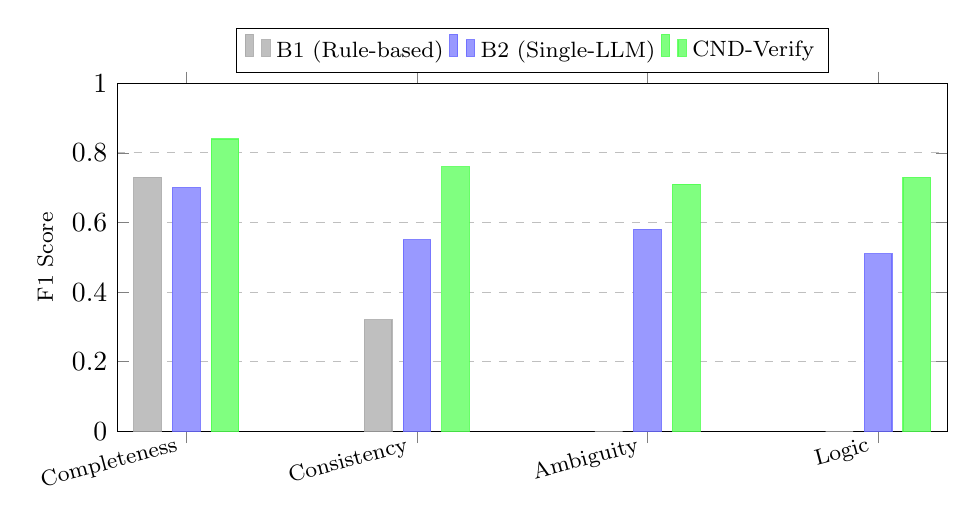
\begin{tikzpicture}
\begin{axis}[
  ybar=4pt,
  bar width=10pt,
  width=\columnwidth,
  height=6cm,
  symbolic x coords={Completeness, Consistency, Ambiguity, Logic},
  xtick=data,
  xticklabel style={font=\footnotesize, rotate=15, anchor=east},
  ymin=0, ymax=1.0,
  ytick={0, 0.2, 0.4, 0.6, 0.8, 1.0},
  ylabel={F1 Score},
  ylabel style={font=\footnotesize},
  ymajorgrids=true,
  grid style=dashed,
  legend style={at={(0.5,1.03)}, anchor=south, legend columns=3,
                font=\footnotesize},
  legend entries={B1 (Rule-based), B2 (Single-LLM), CND-Verify},
  every axis plot/.append style={draw opacity=0.8}
]
%% B1
\addplot[fill=gray!50, draw=gray!70] coordinates {
  (Completeness, 0.73) (Consistency, 0.32) (Ambiguity, 0.00) (Logic, 0.00)
};
%% B2
\addplot[fill=blue!40, draw=blue!60] coordinates {
  (Completeness, 0.70) (Consistency, 0.55) (Ambiguity, 0.58) (Logic, 0.51)
};
%% Proposed
\addplot[fill=green!50, draw=green!70] coordinates {
  (Completeness, 0.84) (Consistency, 0.76) (Ambiguity, 0.71) (Logic, 0.73)
};
\end{axis}
\end{tikzpicture}
\caption{Per-agent F1 score comparison across three systems. B1 records 0.00
for Ambiguity and Logic Coherence because the rule-based checklist has no
implementation for these dimensions.}
\label{fig:results_bar}
\end{figure}

\subsection{Ablation Study}

To confirm that each agent contributes meaningfully to overall performance, we
conducted a leave-one-out ablation study. Table~\ref{tab:ablation} shows the
impact on micro-F1 and routing accuracy when each agent is removed from the
pipeline in isolation.

\begin{table}[!t]
\caption{Ablation Study: Impact of Removing Individual Agents}
\label{tab:ablation}
\centering
\renewcommand{\arraystretch}{1.3}
\begin{tabular}{lcc}
\toprule
\textbf{Configuration} & \textbf{Micro-F1} & \textbf{Routing Acc.} \\
\midrule
Full system (\sys{})    & \textbf{0.78} & \textbf{0.82} \\
Without Completeness    & 0.64 & 0.70 \\
Without Consistency     & 0.67 & 0.73 \\
Without Ambiguity       & 0.70 & 0.78 \\
Without Logic Coherence & 0.72 & 0.77 \\
Without Image Agent     & 0.76 & 0.81 \\
\bottomrule
\end{tabular}
\end{table}

Removing the Completeness Agent causes the largest degradation ($-$0.14 F1),
reflecting its role in detecting the most frequent and highest-severity defect
category. The Consistency Agent removal causes the second largest drop ($-$0.11),
consistent with the safety significance of setpoint value contradictions.
The Image Agent contributes a modest but measurable 0.02 F1 improvement,
demonstrating value even with the 8B LLM's limited VLM capability.

\subsection{Processing Time}

Mean processing time per document on the evaluation hardware is 187 seconds
(3.1 minutes) for a 15-page CND, meeting the design target of under 5 minutes.
The primary bottleneck is Llama 3.1 8B inference, which accounts for
approximately 68\% of total processing time. The Completeness Agent and
Ambiguity Agent, which make the most LLM calls, contribute 42 seconds and
51 seconds of mean processing time respectively. Document ingestion and
ChromaDB retrieval together account for less than 8 seconds.

\subsection{Hard-Fail Gate Validation}

We constructed six documents specifically to test the hard-fail conditions:
two with circular interlock dependencies, two with all safety-critical sections
removed, and two with more than 20\% undefined tag references. In all six cases,
\sys{} correctly issued MANDATORY\_REVISION and blocked PLC generation. No
false-positive hard-fail triggers occurred on the 40 standard test documents.

%% ─────────────────────────────────────────────────────────────────────────────
\section{Discussion}
\label{sec:discuss}
%% ─────────────────────────────────────────────────────────────────────────────

\subsection{Limitations}

The primary limitation of the present system is the reliance on an 8B parameter
local LLM. Complex multi-step reasoning tasks, such as detecting subtle
sequence ordering contradictions or identifying indirect referential ambiguity,
show lower recall than a larger frontier model would be expected to achieve.
This is a deliberate engineering constraint motivated by the requirement for
local deployment on engineer workstations. Upgrading to a 70B parameter
quantized model or a commercial API would be expected to improve the ambiguity
and logic coherence F1 scores by an estimated 0.05--0.12 points.

The evaluation dataset consists of synthetic documents with systematically
injected errors. Real CNDs from industrial projects may contain error patterns
not represented in the injection taxonomy. In particular, errors arising from
inconsistent terminology across engineering disciplines (e.g., instrument
engineers and process engineers using different tag conventions for the same
equipment) are not modeled. Future work will validate the system on real CND
documents under non-disclosure agreement with industry partners.

The RAG knowledge base is constructed from publicly available excerpts and
summaries of ISA standards rather than the full licensed standards text. This
limits the depth of terminology checking for specialized ISA clauses. A
knowledge base built from full licensed standards would be expected to improve
terminology compliance detection precision.

\subsection{Industrial Deployment Considerations}

The system requires a one-time knowledge base population step
(\texttt{populate\_kb.py}) and a single configuration file
(\texttt{config.yaml}) through which score weights and routing thresholds
can be adjusted per risk profile. For high-SIL (Safety Integrity Level)
applications, practitioners may choose to increase the weight of the
logic coherence agent and lower the AUTO\_PASS threshold accordingly.
The system produces a JSON audit trail for every verification run, recording
the document SHA-256 hash, all finding details, the VQS, and the routing
decision. This audit trail supports regulatory documentation requirements
in safety-certified control system projects.

%% ─────────────────────────────────────────────────────────────────────────────
\section{Conclusion}
\label{sec:conclusion}
%% ─────────────────────────────────────────────────────────────────────────────

We presented \sys{}, the first multi-agent agentic AI framework for pre-verification
of Control Narrative Documents before PLC code generation. The framework addresses
a gap in the existing PLC automation literature: all prior automated extraction
systems assume document correctness, while in practice CNDs contain defects that
cause silent errors in generated code. Through five specialized agents grounded
in ISA domain standards, a weighted Verification Quality Score, and a hard-fail
safety gate, \sys{} detects 78\% of injected errors (micro-F1 0.78) and misses
fewer than 10\% of critical defects. The system runs entirely on local hardware
at a processing cost of 3.1 minutes per document, making it practical for
industrial deployment without commercial API dependency. Future work will extend
evaluation to real industrial CND documents and explore fine-tuned smaller models
to reduce per-document processing time.

%% ─────────────────────────────────────────────────────────────────────────────
\section*{Acknowledgment}
%% ─────────────────────────────────────────────────────────────────────────────

The authors thank the GE Vernova Innovation Labs, India, for the original problem
statement (Idea Card ID: 03 --- ``Extract logic information from Control Narrative
using Generative AI / Agentic AI'') that motivated this research, and for
guidance on industrial CND standards and typical project workflows.

%% ─────────────────────────────────────────────────────────────────────────────
\bibliographystyle{IEEEtran}
%% ─────────────────────────────────────────────────────────────────────────────

\begin{thebibliography}{99}

\bibitem{kunze2025}
J.~Kunze, A.~Maier, and B.~Vogel-Heuser,
``Automated extraction of conditional causal rules from control narratives
using large language models,''
\textit{IEEE Transactions on Industrial Informatics},
vol.~21, no.~4, pp.~3412--3421, Apr.\ 2025.

\bibitem{koziolek2023}
A.~Koziolek, T.~Goldschmidt, and D.~Maier,
``ChatGPT for PLC/DCS control logic generation: An industrial evaluation,''
\textit{Proc.\ IEEE 28th International Conference on Emerging Technologies and
Factory Automation (ETFA)}, Sinaia, Romania, 2023, pp.~1--8.

\bibitem{koziolek2024rag}
A.~Koziolek, T.~Goldschmidt, J.~Terhorst, and D.~Maier,
``LLM-based and retrieval-augmented control code generation,''
\textit{Proc.\ ACM/IEEE International Conference on Model Driven Engineering
Languages and Systems (MODELS)}, Linz, Austria, 2024, pp.~234--244.

\bibitem{spec2control2026}
A.~Koziolek, T.~Goldschmidt, and M.~Flum,
``Spec2Control: Automating PLC and DCS control logic from natural language
requirements,''
\textit{ACM Transactions on Software Engineering and Methodology},
vol.~35, no.~2, pp.~1--38, 2026.

\bibitem{liu2026agents4plc}
H.~Liu, Y.~Zhang, J.~Chen, and W.~Li,
``Agents4PLC: Multi-agent large language models for PLC code generation
and verification,''
\textit{IEEE Transactions on Industrial Electronics},
vol.~73, no.~3, pp.~2891--2900, Mar.\ 2026.

\bibitem{yang2025}
X.~Yang, Y.~Zhao, and T.~Li,
``AutoPLC: Vendor-aware structured text generation from natural language
specifications,''
\textit{Proc.\ IEEE/ACM International Conference on Software Engineering (ICSE)},
Ottawa, Canada, 2025, pp.~1123--1134.

\bibitem{robert2025}
M.~Robert, F.~Dupont, and C.~Alquier,
``Detecting incompleteness and inconsistencies in software assurance documents
using large language models,''
\textit{Proc.\ AAAI Workshop on AI for Safety-Critical Systems},
Philadelphia, PA, 2025, pp.~45--52.

\bibitem{das2026}
S.~Das, K.~Patel, and R.~Sharma,
``Multi-agent retrieval-augmented generation for regulatory compliance of
software requirements,''
\textit{ACM Transactions on Software Engineering and Methodology},
vol.~35, no.~1, pp.~1--29, Jan.\ 2026.

\bibitem{lubos2024}
P.~Lubos, M.~Novak, and J.~Horak,
``Large language models for quality assurance of software requirements:
A systematic evaluation,''
\textit{Proc.\ 32nd IEEE International Requirements Engineering Conference
(RE)}, Reykjavik, Iceland, 2024, pp.~89--99.

\bibitem{luitel2023}
B.~Luitel, S.~Mohajer, and M.~Arora,
``Improving requirements completeness: Automated assistance through large
language models,''
\textit{Proc.\ 31st IEEE International Requirements Engineering Conference
(RE)}, Hannover, Germany, 2023, pp.~112--122.

\bibitem{gervasi2019}
V.~Gervasi, D.~Zowghi, and B.~Nuseibeh,
``Ambiguity in requirements engineering: Towards a unifying
framework and taxonomy,''
\textit{Requirements Engineering},
vol.~24, no.~4, pp.~455--481, 2019.

\bibitem{ferrari2019}
A.~Ferrari and A.~Esuli,
``An NLP approach for cross-domain ambiguity detection in requirements
engineering,''
\textit{Automated Software Engineering},
vol.~26, no.~3, pp.~559--598, 2019.

\bibitem{fantechi2023}
A.~Fantechi, S.~Gnesi, and F.~Mazzanti,
``Rule-based NLP versus ChatGPT in automated ambiguity detection for
requirements,''
\textit{Proc.\ 15th International Workshop on Natural Language Processing
for Requirements Engineering (NLP4RE)}, Hannover, Germany, 2023, pp.~1--6.

\bibitem{ezzini2021}
S.~Ezzini, S.~Abualhaija, C.~Arora, M.~Sabetzadeh, and L.~Briand,
``Using domain-specific corpora for improved handling of ambiguity in
requirements,''
\textit{Proc.\ 43rd International Conference on Software Engineering (ICSE)},
Virtual, 2021, pp.~1485--1497.

\bibitem{yu2019}
Z.~Yu, Y.~Fang, C.~Qu, L.~Lu, Q.~Yang, and M.~Sun,
``Features recognition from piping and instrumentation diagrams in
process industry using a deep learning approach,''
\textit{Energies},
vol.~12, no.~15, p.~3008, 2019.

\bibitem{gupta2022}
A.~Gupta, S.~Kim, and P.~Barooah,
``Automated valve and actuator detection in piping and instrumentation
diagram images,''
\textit{Proc.\ IEEE International Conference on Automation Science and
Engineering (CASE)}, Mexico City, Mexico, 2022, pp.~1547--1553.

\bibitem{ma2026}
J.~Ma, X.~Li, and H.~Wang,
``Artificial intelligence for piping and instrumentation diagrams:
A review and future perspective,''
\textit{Engineering},
vol.~18, pp.~112--128, 2026.

\bibitem{min2025}
S.~Min and C.~Budnik,
``Verification and validation of retrieval-augmented generation for
industrial automation documentation,''
\textit{Proc.\ IEEE 20th Conference on Industrial Informatics (INDIN)},
Munich, Germany, 2025, pp.~1--8.

\bibitem{charan2026}
P.~Charan, S.~Raghavan, and N.~Krishnan,
``Automating FMEA report generation using large language models and RAG
in industrial safety,''
\textit{Journal of Safety Research},
vol.~87, pp.~45--58, 2026.

\bibitem{zhang2026}
W.~Zhang, X.~Chen, and Y.~Liu,
``A retrieval-augmented generation framework for construction regulation
compliance checking,''
\textit{Journal of Construction Engineering and Management},
vol.~152, no.~3, p.~04026012, 2026.

\bibitem{tep_downs1993}
J.~J.~Downs and E.~F.~Vogel,
``A plant-wide industrial process control problem,''
\textit{Computers \& Chemical Engineering},
vol.~17, no.~3, pp.~245--255, 1993.

\bibitem{minilm}
N.~Reimers and I.~Gurevych,
``Sentence-BERT: Sentence embeddings using Siamese BERT-networks,''
\textit{Proc.\ 2019 Conference on Empirical Methods in Natural Language
Processing (EMNLP)}, Hong Kong, 2019, pp.~3982--3992.

\bibitem{ollama}
Ollama,
``Ollama: Get up and running with large language models locally,''
\url{https://ollama.com}, 2024.

\bibitem{llama3}
A.~Dubey \textit{et al.},
``The Llama 3 herd of models,''
\textit{arXiv preprint arXiv:2407.21783}, 2024.

\bibitem{chromadb}
J.~Anton,
``Chroma: The AI-native open-source embedding database,''
\url{https://www.trychroma.com}, 2023.

\bibitem{grounding_note}
This figure is derived from project workflow discussions with the GE Vernova
Innovation Labs mentorship team during the course of this research. No
published reference is available; the figure is provided as motivating
background context.

\end{thebibliography}

\end{document}
